\chapter{Functionality Index}

\section{Manipulating Geometrical Data}

There is a small number of function to manipulate geometric data in \ogs. The common approach to the manipulation of \ogs input data is that it should be changed in a GIS or other specialised software of the user's choice which usually offers much more functionality for these things than \ogs ever could.

Functions for the manipulation of geometric data that \emph{are} implemented are all associated with polylines and can be applied by right-clicking the ``Polylines'' item of any geometry and selecting \cmd{Connect Polylines...}.

\subsubsection{Connecting Polylines}
This function connects all the selected polylines to a single new polyline provided that the start- and end points of all segments are within the given maximum distance. The default maximum distance is $0.0$, meaning that start- and end points have to be identical.

Note that if more than two start/end points are located within the given maximum distance, still only two of those points are connected. These points are chosen randomly.

\subsubsection{Creating Polygons by Closing Polylines}
This function closes a (connected) polyline. Simply check `Close connected Polyline'. If a name has been entered, this name will be assigned to the closed polyline.

\subsubsection{Creating Surfaces by Triangulating Polygons}
This function additionally creates a new surface by triangulating the polygon. This simply requires checking `Create Surface from Polyline'. The newly created polyline has to be closed for that function to work. If a name has been entered, this name will be assigned to the surface.

\section{Creating Meshes from Geometry}

By selecting \cmd{Tools\ra Mesh Generation...} you open a dialog that allows you to create meshes using information currently present in the programme. For this to work you have to have GMSH\footnote{http://geuz.org/gmsh/} installed and be available from the location of the Data Explorer.

Specifically, you can select any geometry and observation sites that should be considered for generating the mesh. Note that all points of every data set considered for mesh generation will be included as nodes in the final mesh. Upon pressing \cmd{OK} a geometry-file for GMSH is written, GMSH is called to create the mesh and the newly created mesh is at once imported in the \ogs-Data Explorer.

There is an \cmd{Advanced}-Tab in this dialog that allows you set a number of parameters for the mesh. Most importantly you can select if you want an adaptive mesh or a homogeneous mesh. An adaptive mesh is refined towards points or lines specified in the geometry while a homogeneous mesh has elements of roughly the same size everywhere in the domain (see figure \ref{fig:meshing}).

\begin{figure}[tb]
\begin{center}
\subfloat[Geometry]{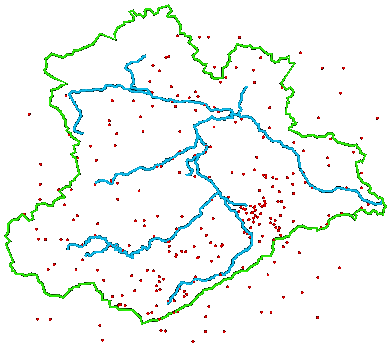
\includegraphics[width=0.3\linewidth]{meshing-geo}\label{meshing-geo}}\enspace
\subfloat[Homogeneous mesh]{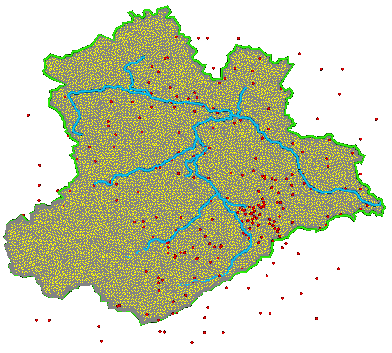
\includegraphics[width=0.3\linewidth]{meshing-hmg}\label{meshing-hmg}}\enspace
\subfloat[Adaptive mesh]{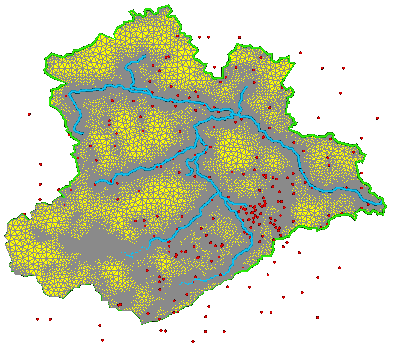
\includegraphics[width=0.3\linewidth]{meshing-adp}\label{meshing-adp}}
\end{center}
\caption{Meshing using geometric data and observation sites.} \label{fig:meshing}
\end{figure}

The specific parameters for adaptive meshes are:
\begin{itemize}
\item \textbf{Max. number of points in Quadtree leaf:} Generally speaking, the smaller this number the finer will the resulting mesh be. \\
    To be more exact, you have to have a basic idea what a quad tree \footnote{http://en.wikipedia.org/wiki/Quadtree} is. A tree structure is constructed by a sequential subdivision of the domain based on the distribution of relevant points in space. The criterium if a segment compromising a leaf is further refined is dependent on the number of points located in that segment. Therefore, larger numbers of that parameters will usually result in coarser meshes while smaller numbers will result in finer meshes. \emph{Note that this is technically not a correct explanation as results are heavily dependent on how many points are located in certain sub-divisions of the domain, the existence of point clusters, etc.}
\item \textbf{Mesh density scaling for points:} This is a scaling factor for the above parameter allowing for a refinement towards points located within the outer boundary. In general, smaller values will result in finer meshes.
\item \textbf{Mesh density scaling for stations:} This is exactly the same kind of scaling factor as for the option above, only for refinement towards observation sites.
\end{itemize}

Likewise, you can select an \textbf{Element Size} for homogeneous meshes. Here, too, a smaller number will result in a finer mesh.

\bigskip

Default parameters for all options are already predefined and have worked well with most examples that have been tested. Feel free to play around with these numbers but realise that the resulting mesh might not be what you have in mind.

\section{Analyse Mesh Quality}

You can visualise the quality of a given mesh by right-clicking on the mesh in the respective data view and selecting \cmd{Check Mesh Quality...}. This gives a colour-codes overlay of the mesh where every element is assigned a quality in $[0,1]$. You can select this overlay in the visualisation pipeline and specify thresholds to select a certain range of quality and see which element fall into that range. \textit{(Note: You might need to manually set the correct scalar array for visualising mesh quality. The appropriate data can be chosen by selecting in ``C-Selection'' in the \cmd{Active Scalar} pull-down menu.}

The currently implemented measure analyses the ratio of shortest to longest edge of every element. This is a pretty good measure for triangle elements but might be not as good as others. Also, the quality measure you need might depend on the process you want to simulate with your mesh.

Additional options for measurements of mesh quality (e.g. based on volume or angles) will be implemented in the future.

\section{Time series data and stratigraphic data}

For observation sites it is possible to display additional information such as logger data at the site or the stratigraphy at a borehole. Both features are currently only implemented as a proof of concept and need to be expanded in the future.

To view the additional information of an observation site load a stn-file into the programm and right-click on any observation site in the data view. You will see either the menu entry ``View Stratigraphy...'' for a borehole or ``View Diagram...'' for a station. If you selected to view a diagram, a dialog will open which allows you to select a start and end date or to load a file that contains the data (if no associated data base entry for the station has been found). A new window will open, displaying the requested information.

\section{Visualisation Properties}

You can change some properties of the render window by clicking \cmd{Settings\ra} \cmd{Visualisation Settings...}. The dialog that opens allows you to change the background colour of the render window as well as some small changes concerning the illumination of the scene.

For any rendered scene a light source has to be specified (basically the equivalent to the sun or a lamp in the room). Per default this light source is identical with the viewer, i.e. the light source always illuminated the part of an object in the render window that can be seen by the user. In some cases this illumination is not enough, though, and certain parts of a rendered object may be shrouded in darkness. Therefore it is possible to switch on additional light sources above and below the object to ensure a full illumination of the scene.

A global superelevation factor can be applied to all root objects in the visualisation pipeline. This overwrites all previously set superelevation factors.

Per default on loading new data the 3D view is adapted to show the entire scene. This can be switched of (e.g. useful for making a series of screenshots).

\section{General Visualisation Options}
\label{genvisoptions}

For each object in the visualisation pipeline there a number of parameters that can be changed to make the object more easily distinguishable or to convey information contained in the data.

\begin{figure}[tb]
\begin{center}
\subfloat[Solid Color]{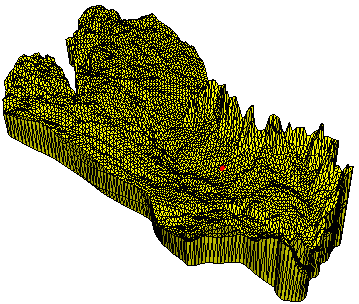
\includegraphics[width=0.3\linewidth]{colour-solid}\label{colour-solid}}\enspace
\subfloat[Default colour table]{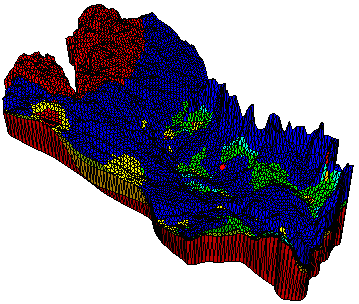
\includegraphics[width=0.3\linewidth]{colour-default}\label{colour-default}}\enspace
\subfloat[User-defined colours]{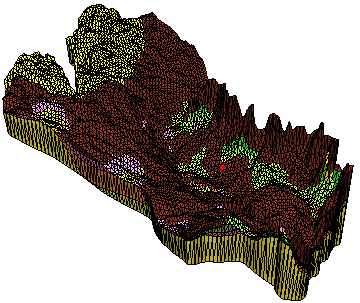
\includegraphics[width=0.3\linewidth]{colour-user}\label{colour-user}}
\end{center}
\caption{Each object is assigned a random solid colour as well as a default colour table based on a temperature scale (from blue to red). The solid colour can be adjusted via the ``Diffuse Color''-option (see section \ref{genvisoptions}), the colour table can be adjusted by loading a user-defined *.lut file via the ``Add color table...''-option (see section \ref{specvisoptions}).} \label{fig:colours}
\end{figure}

In detail these parameters are:

\begin{itemize}
\item Diffuse Color: Each item is assigned a colour which is used for rendering the object in 3D space. This colour can be changed here (see figure \ref{colour-solid}).
\item Active Scalar: Each visualisation object has an assigned colour which is used in the rendering process (see above). However, some data sets contain additional information (e.g. material groups for meshes, concentration of chemical substances, etc.). This information can be selected here and is then employed in the rendering of object in the render window (see figure \ref{colour-default}).
\item Visible Edges: Some objects (such as meshes) are composed of a combination of lines (edges) and surfaces. While the colour of the surfaces can be set using the \emph{Diffuse Color}-button, the colour of the edges can be changed here. Furthermore the rendering of edges can be switched off by unchecking the box next this option.
\item Opacity: Determines if an object appears to be transparent or not.
\item Scaling Factor: Super-elevates the data by the given factor. This makes it much more easy to recognise differences in height.
\end{itemize}

\section{Object-specific Visualisation Options}
\label{specvisoptions}

There are a number of options that are available only for certain types of data. These options can be selected by right-clicking on an item in the visualisation pipeline.

\begin{itemize}
\item \textbf{Add filter...:} Allows to apply a filter to the current objects. For details on that option see section \ref{filters}.
\item \textbf{Add color table...:} Allows you to assign a specific colour table to the currently selected scalar array. The colour table is loaded from a *.lut-file (see figure \ref{colour-user}).\\
    This option is available for all objects except image data.
\item \textbf{Convert to Mesh...:} Allows to convert an object of the VTK-data type ``Unstructured Grid'' to be converted into an \ogs mesh. Objects of that type are basically meshes that are contained in different data structure than ``normal'' \ogs meshes. Therefore, this specifically allows the conversion of imported VTK-files to \ogs meshes.\\
    This option is available for all objects of type ``VTK\_UN\-STRUCT\-URED\_GRID'' (i.e. all mesh objects).
\item \textbf{Convert Image to Mesh...:} Generates an \ogs mesh based on a given raster file. Specifically, the result is mesh built from rectangular equilateral triangle elements, with two triangles forming on square (this is basically a representation of the pixels of the raster file). If the raster file contains ``NoData''-values (e.g. raster files created with a Geographic Information System), these values are ignored. See figure \ref{Filter-Img4}.\\
    This options is only available for image data (i.e. raster files).
\item \textbf{Export to VTK:} All objects displayed the render window are technically VTK-objects. Choosing this option saves these objects in VTK-format to a file. They can then be used in any software supporting this format (e.g. Paraview\footnote{http://www.paraview.org/}).
\item \textbf{Export to OpenSG:} Converts objects into OpenSG format (*.osg). This is another open source graphics format. It is also the format used by the UFZ VisLab. Specifically, this also implies that \emph{anything} that can be visualised in \ogs can also be exported to OpenSG and be presented in the VisLab.
\end{itemize}

\section{Applying Filters for Visualisation}
\label{filters}

In contrast to the options detailed in the previous section, filters are a manipulation of the actual graphics object to enhance, reduce or deform certain aspects of these objects for imparting information that might not be superficial\footnote{One might argue that this definition also holds true for the assignment of specific color tables which is accessed via right-click on an object. This inconsistency originates in the data structures the objects are stored in and in defining an easy-to-use workflow for using this functionality.}.

To apply a filter, right-click on an object in the visualisation pipeline and select \cmd{Add filter...}. A dialog will pop up which lets you select one of a number of available filters. As before, filters will only be displayed for objects they can be applied to. However, this does not mean that it makes sense to apply any filter to any object where it can be applied. Also note, that it is possible (and sometimes useful) to apply filters to filters to extract certain information bit by bit.
%
\begin{figure}[tb]
\begin{center}
\subfloat[Raster data]{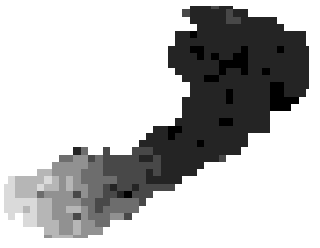
\includegraphics[width=0.4\linewidth]{Filter-Img1}\label{Filter-Img1}}\enspace
\subfloat[Apply lookup table to image]{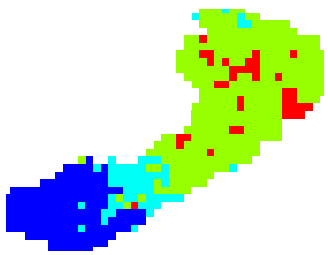
\includegraphics[width=0.4\linewidth]{Filter-Img2}\label{Filter-Img2}} \\
\subfloat[Image to bar chart]{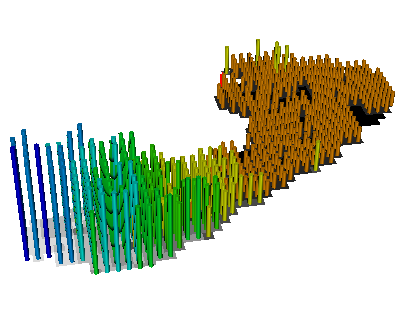
\includegraphics[width=0.4\linewidth]{Filter-Img3}\label{Filter-Img3}}\enspace
\subfloat[Convert Image to Mesh]{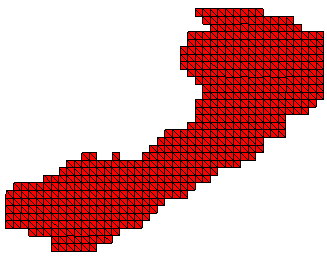
\includegraphics[width=0.4\linewidth]{Filter-Img4}\label{Filter-Img4}}
\end{center}
\caption{\ogs functionality applicable to image-/raster-data.} \label{fig:filter:raster}
\end{figure}
%
All available filters will be detailed in the following.

\subsubsection{Apply lookup table to image}
\bstart{Applicable to:} Image Data

\bstart{Effect:} Applies default color table to images, replacing grey values with a temperature scale (i.e. dark colours are blue, light colours are red). This results in an image where certain gradients are much better discernable. See figure \ref{Filter-Img2}.

\bstart{Remarks:} \emph{This is similar to applying a pre-defined colour table to a geometry- or mesh object. The implementation as a filter for images is based on the very different structure of image objects in the graphics library VTK which is used for visualisation.}

\begin{figure}[tb]
\begin{center}
\subfloat[Geometry Data]{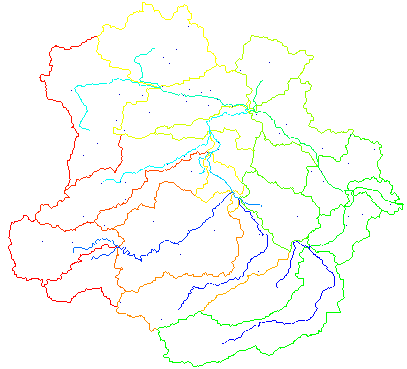
\includegraphics[width=0.4\linewidth]{Filter-Poly1}\label{Filter-Poly1}}\enspace
\subfloat[Points to Spheres]{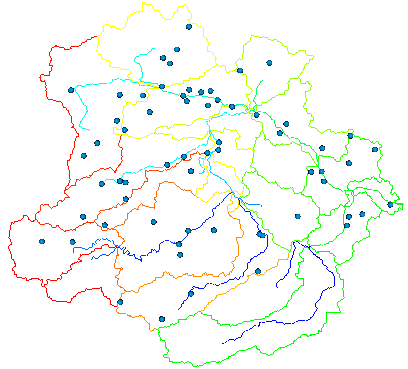
\includegraphics[width=0.4\linewidth]{Filter-Poly2}\label{Filter-Poly2}} \\
\subfloat[Lines to tubes]{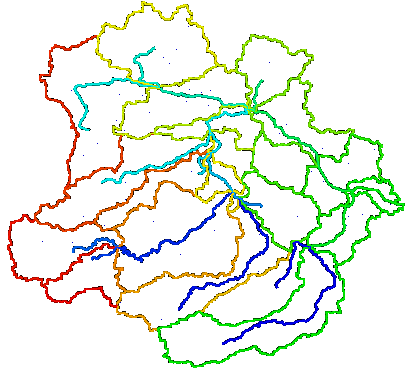
\includegraphics[width=0.4\linewidth]{Filter-Poly3}\label{Filter-Poly3}}\enspace
\subfloat[Extract cells by threshold]{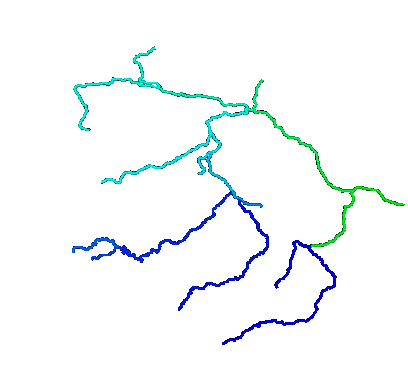
\includegraphics[width=0.4\linewidth]{Filter-Poly4}\label{Filter-Poly4}}
\end{center}
\caption{\ogs functionality applicable to geometry data. In figure \ref{Filter-Poly2} ground water stations in the area have been emphasised. In figure \ref{Filter-Poly4} a threshold filter has been applied to the tube-filtered data from figure \ref{Filter-Poly3} to select only the river network of the depicted area from the geometric data.} \label{fig:filter:poly}
\end{figure}

\subsubsection{Apply texture to surface}
\bstart{Applicable to:} Surfaces, Meshes

\bstart{Effect:} Allows to map an image/raster on a surface or mesh. This might be additional information such as land use classes, precipitation, etc. See figure \ref{Filter-Mesh4}.

\subsubsection{Elevation-based colouring}
\bstart{Applicable to:} Geometry, Meshes

\bstart{Effect: } Applies a colour to each point depending on the z-coordinate of that point, assuming that this denotes height in metres. The pre-defined colour scale starts with blue up to a height of $0$ metres (i.e. sea level), which is then slowly changing to green (150\,m) and yellow (450\,m) and then changing to red from then on. See figure \ref{Filter-Mesh2}.

\bstart{Remarks:} \emph{In theory these values can be changed. This is, however, currently not possible using the GUI.}

\begin{figure}[tb]
\begin{center}
\subfloat[Multilayered Mesh]{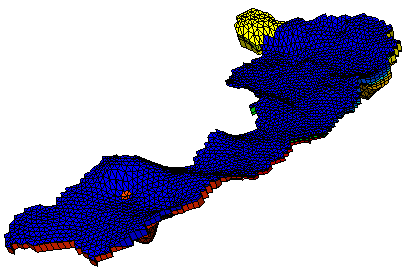
\includegraphics[width=0.4\linewidth]{Filter-Mesh1}\label{Filter-Mesh1}}\enspace
\subfloat[Elevation-based colouring]{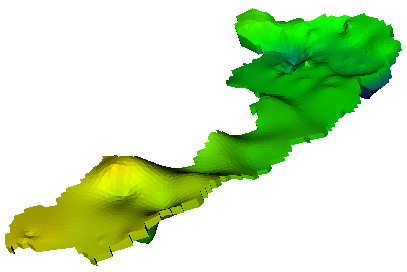
\includegraphics[width=0.4\linewidth]{Filter-Mesh2}\label{Filter-Mesh2}} \\
\subfloat[Extract cells by threshold]{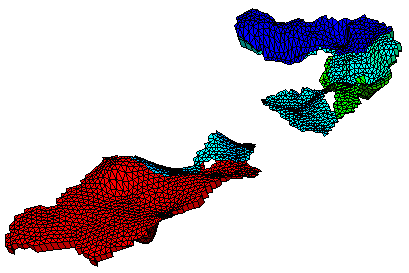
\includegraphics[width=0.4\linewidth]{Filter-Mesh3}\label{Filter-Mesh3}}\enspace
\subfloat[Apply texture to surface]{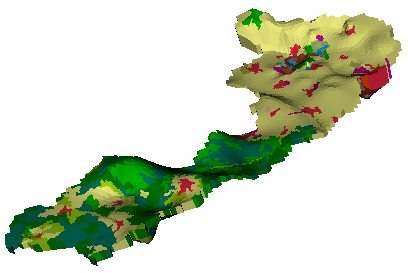
\includegraphics[width=0.4\linewidth]{Filter-Mesh4}\label{Filter-Mesh4}}
\end{center}
\caption{\ogs functionality applicable to meshes.} \label{fig:filter:mesh}
\end{figure}

\subsubsection{Extract cells by threshold}
\bstart{Applicable to:} Lines, Surfaces, Meshes

\bstart{Effect:} Each line, surface and mesh layer has a unique ID which allows to assign different colours to different objects. This filter furthermore allows to select a range of objects which should be displayed while all other objects are blanked out. This way you can visualise only a specified stratigraphic layer or a certain polyline, etc. See figures \ref{Filter-Poly4} and \ref{Filter-Mesh3}.

\subsubsection{Image to bar chart}
\bstart{Applicable to:} Image Data

\bstart{Effect:} Each pixel is assigned a bar depending on the grey value of the pixel. Also, the colour changes of that bar changes according to its height. See figure \ref{Filter-Img3}.

\bstart{Remarks:} \emph{This filter takes a lot of time for large images as the result becomes very complex. The intention is to use it for low resolution raster data of phenomena such as precipitation, etc.}

\emph{This is a good example on the combination of the successive application of these filters. This one combines `Image to vertical lines', `Lines to tubes' and `Elevation-based colouring'.}

\subsubsection{Image to vertical lines}
\bstart{Applicable to:} Image Data

\bstart{Effect:} Plots vertical lines for every pixel of a raster with each line having a height depending on the raster's grey value.

\bstart{Remarks:} \emph{This is a filter that is needed for the correct application of other filters. It is probably not of much use on itself.}

\subsubsection{Lines to tubes}
\bstart{Applicable to:} Geometry, Observation sites

\bstart{Effect:} A geometric line has independent of the current zoom level always a thickness of $1$. This filter allows to assign a `real' thickness to line-objects that also changes according to the current zoom. See figure \ref{Filter-Poly3}.

\subsubsection{Points to spheres}
\bstart{Applicable to:} Geometry, Observation sites

\bstart{Effect:} A geometric point has independent of the current zoom level always a diameter of $1$. This filter allows to assign a `real' diameter to point-objects that also changes according to the current zoom. See figure \ref{Filter-Poly2}.

\subsubsection{Surface filter}
\bstart{Applicable to:} Meshes

\bstart{Effect:} Extracts the outer surface of a mesh.

\bstart{Remarks:} \emph{This is a filter that is needed for the correct application of other filters. It is probably not of much use on itself.}
